\documentclass[10pt,a4paper,twocolumn]{article}

\usepackage[a4paper,top=1.75cm,bottom=2.0cm,left=1.75cm,right=1.75cm,columnsep=0.65cm]{geometry}
\usepackage{times}
\usepackage[T1]{fontenc}
\usepackage[utf8]{inputenc}
\usepackage{microtype}
\usepackage{amsmath}
\usepackage{booktabs}
\usepackage{tabularx}
\usepackage{enumitem}
\usepackage{xcolor}
\usepackage{graphicx}
\usepackage{natbib}
\usepackage{tikz}
\usetikzlibrary{arrows.meta,positioning,fit,backgrounds}
\usepackage[hidelinks]{hyperref}
\usepackage{titlesec}

\setlength{\parindent}{1em}
\setlength{\emergencystretch}{1.6em}
\setlength{\parskip}{0pt}
\setlength{\textfloatsep}{8pt plus 2pt minus 2pt}
\setlength{\floatsep}{7pt plus 2pt minus 2pt}
\setlength{\intextsep}{7pt plus 2pt minus 2pt}
\setlist{nosep,leftmargin=1.4em}
\titleformat{\section}{\large\bfseries}{\thesection}{0.55em}{}
\titleformat{\subsection}{\normalsize\bfseries}{\thesubsection}{0.45em}{}
\titlespacing*{\section}{0pt}{1.4ex plus .4ex}{0.7ex}
\titlespacing*{\subsection}{0pt}{1.0ex plus .3ex}{0.4ex}
\graphicspath{{../figures/}{./}}

\newcommand{\tabnote}[1]{\par\vspace{1pt}{\footnotesize #1}}

\title{Reproducing LLMLingua: Evaluating Accuracy--Efficiency Trade-offs in Long-Context Prompt Compression}

\author{
CHEN IAT HONG \quad MC654102\\
KONG KIN MENG \quad MC652817\\
CHE CHON HONG \quad MC551841\\
\textit{University of Macau}\\
\textit{CISC7021 Applied Natural Language Processing -- Course Project Final Report}
}

\date{}

\begin{document}
\maketitle
\vspace{-0.8cm}

\begin{abstract}
Long prompts improve retrieval-augmented and in-context question answering, but
they also raise memory use, latency, and cost, and models may ignore information
placed in the middle of a long context. Prompt compression attacks both problems
without retraining the target model, yet its reported gains are usually measured
with proprietary LLMs and reported as token reductions rather than end-to-end
cost. We implement and evaluate four prompt settings on the full 150-example
LongBench \texttt{multifieldqa\_en} split with a 3B open-weight target model:
an uncompressed baseline, head-and-tail truncation, LLMLingua, and a
question-aware long-context variant of LLMLingua, the last two at nominal $2\times$
and $4\times$ compression. All settings share one fixed sample index, one prompt
template, and one Exact Match / token-F1 implementation. Historical mean F1 decreases across the two requested settings in every compressed family. Truncation
keeps most of the baseline quality (F1 0.4065 and 0.3620 against 0.4296), whereas
LLMLingua is markedly worse (0.2626 and 0.2207); replacing its chunked Phi-2
compressor with a single-pass question-aware compressor recovers part of the loss
(0.3070 and 0.2794) but still falls short of truncation, the goal it was designed to reach. In a same-machine rerun of
the first three settings, only truncation actually reduces end-to-end latency, by
44\% and 66\%, while LLMLingua at $2\times$ is 44\% slower than the uncompressed
baseline despite removing half of the prompt tokens. A later full-split released-recipe Alpaca evaluation also favors truncation at actual matched budgets (F1 0.2396/0.2174 versus 0.3875/0.3494); it is separate from the historical runs. A position analysis of the
truncation errors shows that the share of approximate gold-answer locations in the removed middle increases from 21\% to 37\%. This association does not establish a causal decomposition of the accuracy loss.
\end{abstract}

% ---------------------------------------------------------------------------
\section{Introduction}

\subsection{Motivation}

Large language models (LLMs) are now routinely asked to answer a question from
several retrieved documents, to summarise a long article, or to learn a task from
many in-context demonstrations. Each of these settings pushes thousands of tokens
into a single prompt. The cost is not only monetary: a longer prompt occupies more
GPU memory, needs more prefill computation, and therefore increases the
time-to-first-token and the end-to-end latency of the serving system. Retrieved
context is also repetitive. Documents overlap with one another and with the
instruction, so a non-trivial fraction of the prompt carries little new
information for the question at hand. Finally, a large advertised context window
does not imply that the model uses it uniformly: \citet{liu-etal-2024-lost} show
that accuracy is typically highest when the relevant passage sits at the
beginning or the end of the context and drops when it sits in the middle.

Prompt compression addresses these issues by shortening the text that reaches the
target model while trying to preserve the information the task needs. Unlike
model compression or distillation, it requires neither retraining nor access to
the target model's weights, so a compressor can be placed before a compatible open or proprietary endpoint. This makes it an attractive engineering option for
resource-constrained deployments, and it is the reason a family of
perplexity-based methods has been developed around it.

What is missing is not a new method but a clean measurement. The headline numbers
in this literature are typically obtained with proprietary target models and are
reported as reductions in input tokens. Token reduction, however, is only one side
of the ledger: the compressor itself is a language model that must run on the same
hardware, and its cost can exceed the generation time it saves. It is therefore
unclear whether the accuracy--efficiency trade-off reported for large proprietary
models still holds for a smaller open-weight model that a student project, or a
small deployment, can actually afford to run---and whether the compressor pays for
itself once its own latency is counted.

\subsection{Literature Review}

\citet{li-etal-2025-prompt-survey} organise the field and separate methods that
delete or rewrite visible prompt tokens from methods that encode the prompt into
learned continuous representations. The former are directly applicable to any
frozen model and are the family studied here.

Selective Context \citep{li-etal-2023-compressing} removes lexical units whose
self-information is low, showing that natural-language prompts contain
substantial redundancy. Its importance estimate is not conditioned on the
downstream question, so it may discard details that are predictable in general but
essential for a specific query.

LLMLingua \citep{jiang-etal-2023-llmlingua} introduces a coarse-to-fine framework
in which a small language model scores prompt components and individual tokens.
A budget controller first allocates different compression budgets to instructions,
demonstrations, and questions; iterative token-level compression then removes
low-value tokens in several passes, and distribution alignment reduces the gap
between the compressor and the target model. Reported gains reach roughly
$20\times$ compression with limited quality loss on some tasks.

LongLLMLingua \citep{jiang-etal-2024-longllmlingua} extends the idea to
long-context question answering, where useful evidence is sparse and
question-dependent. It adds question-aware document ranking, contrastive
perplexity, dynamic budget allocation, document reordering, and subsequence
recovery, and reports large token and cost savings on a multi-document Natural
Questions variant \citep{kwiatkowski-etal-2019-natural}.

Two evaluation resources complete the picture. \citet{liu-etal-2024-lost} motivate
the accuracy side of our measurement by documenting position bias, and LongBench
\citep{bai-etal-2024-longbench} supplies the long-context question-answering data
we use, in a format that requires no additional preprocessing.

\subsection{Research Questions}

We ask three questions about a small, reproducible configuration:

\begin{itemize}
    \item \textbf{RQ1:} How does the compression ratio affect question-answering
    accuracy?
    \item \textbf{RQ2:} At the same input-token budget, does LLMLingua outperform
    simple truncation?
    \item \textbf{RQ3:} Does compression reduce end-to-end latency once the
    compression overhead is included?
\end{itemize}

\subsection{Contributions}

\begin{itemize}
    \item A shared evaluation harness, used unchanged by all four experiments: one
    fixed index of the 150 official \texttt{multifieldqa\_en} test examples, one
    chat-template prompt renderer, one set of Exact Match / token-F1
    implementations, and one configuration module.
    \item Four compression settings implemented end to end and run to completion on
    the full split: uncompressed, head-and-tail truncation, LLMLingua, and a
    question-aware long-context variant of LLMLingua, the latter two at nominal
    $2\times$ and $4\times$ compression (seven result settings in total).
    \item A paired, per-sample comparison with 95\% confidence intervals, which is
    more informative than comparing leaderboard averages and lets us state
    explicitly which differences survive noise.
    \item A single-machine rerun of the five uncompressed/truncation/LLMLingua
    settings, so that the latency question (RQ3) is answered on one GPU rather
    than by comparing four different machines.
    \item A negative result: LLMLingua loses to plain truncation at a comparable token budget, and Part 4, which was designed to overtake truncation, recovers 31--42\% of the observed gap while changing several factors together. The contribution of chunking alone is not identified.
    \item A token-offset answer-position analysis of the truncation baseline that
    localises where its errors come from, and a set of reproducible qualitative
    cases for LLMLingua.
\end{itemize}

% ---------------------------------------------------------------------------
\section{Detailed Description}

Our design freezes downstream evaluation so that method differences can be examined. Hardware and implementation differences remain explicit limitations. The project therefore separates a
\emph{frozen} evaluation contract (data, prompt wording, metrics, decoding
parameters) from four \emph{replaceable} compression components. Each component is
a drop-in stage that maps a document set and a question to a (possibly shorter)
prompt; everything downstream of that stage is shared. Seven result settings are
produced in the historical comparison: one uncompressed baseline and three compressed families at two nominal ratios, all evaluated on the same 150 samples in the same order. The later released-recipe experiment is reported separately.

\subsection{Task and Dataset}

We use \texttt{multifieldqa\_en} from LongBench \citep{bai-etal-2024-longbench},
an English single-document question-answering task. Each example contains a question, one long article drawn from diverse sources (LaTeX papers, legal documents, government reports and web PDFs), and one gold answer string in each of the 150 evaluated examples. Three properties made it suitable for this project. First, it
requires no preprocessing: the official JSONL already provides a single
concatenated \texttt{context} field and a \texttt{question} field, so all four
implementations consume exactly the same text. Second, its prompts are genuinely
long: in our chat-templated form the mean prompt is 6{,}966.8 tokens and the
median is 7{,}023 and the longest is 15{,}026, which is long enough for compression to matter and short
enough to run on a single 12--16\,GB GPU. Third, the gold answers are short
free-form strings, which the standard Exact Match and token-F1 implementations can
score without a judge model.

We evaluate on the \emph{complete} official test split of 150 examples rather than
a subsample. A subsample would have introduced a second source of variance on top
of the compression effect, and 150 examples already keep the standard error of a
mean F1 near 0.024, which is small enough for the paired contrasts we report. The
sample identifiers are stored once in \texttt{shared/samples.json} in a fixed
order derived from seed 42, and every result file is checked against that list.

One property of the dataset matters for interpretation. Many gold answers are
annotator-written sentences rather than verbatim spans of the context, so a
case-insensitive literal search recovers the answer string in only 18 of the 150 samples. This
inflates the difficulty of Exact Match (a model must reproduce the full sentence
to score 1) and it is why our answer-position analysis in
Section~\ref{sec:position} relies on normalised matching plus a fuzzy fallback.

\subsection{Models and Hardware}

\paragraph{Target model.} All generation uses Llama-3.2-3B-Instruct. The canonical
identifier \texttt{meta-llama/Llama-3.2-3B-Instruct} is licence-gated on the
Hugging Face Hub, so we load the released mirror
\texttt{unsloth/Llama-3.2-3B-Instruct}. The model is natively a 128k-context model
(\texttt{max\_position\_embeddings} $=131072$ with Llama-3 RoPE scaling), so no
sample in the split exceeds its window. We nevertheless impose a prompt budget of
32{,}768 tokens (32{,}672 after reserving 64 generation tokens and 32 tokens of
margin). The cap exists only to bound the fp16 KV cache on a 12\,GB card; the
longest prompt uses less than half of it, and the recorded
\texttt{truncated\_samples} count is 0 for the baseline, which is what an
``uncompressed'' reference must be able to claim.

\paragraph{Compressors.} Part 3 uses \texttt{microsoft/phi-2} (2.7B) as the
LLMLingua compressor, the option documented by the official project. Part 4
replaces it with \texttt{Qwen2.5-1.5B-Instruct} loaded in 4-bit precision, which
provides a much longer working context and supports question-conditioned
compression. Because the compressor and the target model use different tokenizers,
the historical Phi-2 compressor uses \texttt{NousResearch/Llama-2-7b-hf} to allocate its internal budget. Every reported target prompt length and whole-prompt ratio instead uses the Llama-3.2 tokenizer, so the comparison is in target-token units.

\paragraph{Hardware.} The four parts ran on four machines: a local RTX 3060
(Part 1), a Colab Tesla T4 in fp16 (Part 2), an Apple M5 Pro GPU through MPS
(Part 3), and a Colab CUDA GPU (Part 4). The shared prompts and scoring support an accuracy comparison, but greedy decoding is not bit-exact across environments. Direct latency comparisons require common hardware because the same prompt takes different times on these devices. We
therefore added a fifth experiment that replays the five
uncompressed/truncation/LLMLingua settings back to back on the RTX 3060 with a
single environment and separate stage subprocesses, and every latency claim in this report comes from that rerun.
Part 4 has no such counterpart, because its compressor could not be loaded on that
host; its timings are reported separately and never compared with the rerun.

\subsection{Shared Evaluation Harness}

The harness is a small Python package, \texttt{shared/}, containing four modules:
\texttt{samples.json} (the 150 examples in fixed order), \texttt{config.py} (model
identifiers, token budgets, decoding parameters), \texttt{prompt\_template.py}
(prompt rendering and budget-aware construction) and \texttt{metrics.py} (Exact
Match and token F1). Nothing in this package may be modified by an individual
member; a change requires a group decision, because a single altered prompt
delimiter or token budget silently invalidates all cross-method comparisons. Each
member contributes a runner that consumes the package and writes one JSON record
per sample.

\subsubsection{Sample Index}

The index is a list of 150 identifiers in a fixed order, generated once with seed
42 from the official split and frozen in version control. It does three things: it
guarantees that all four methods answer the same questions, it fixes the iteration
order so that resume logic and chunked schedules are reproducible, and it makes
the paired statistical test possible, since a paired difference is only defined
for two scores of the same item. We verified after every run that each result file
contains exactly the 150 identifiers, in matching membership and without
duplicates; all five per-part result files pass this check.

\subsubsection{Prompt Template}

Prompt wording follows the official LongBench template: a short system message
(``answer questions based only on the provided text'') and a user message of the
form \emph{Read the following text and answer the question briefly. / Text: \dots
/ Question: \dots / Answer:}. Prompts are built by applying the model's chat
template with \texttt{add\_generation\_prompt=True} and are then tokenised with
\texttt{add\_special\_tokens=False}, so the recorded \texttt{prompt\_tokens} is
the token count of the exact rendered prompt the model consumes, not the length of a
proxy string. This matters for the ratio accounting: a compressor removes document
tokens only, and the instruction and question are unchanged across settings. Tokenization at concatenation boundaries can still affect exact counts.

For the uncompressed baseline we additionally implement a budget fallback: if a
prompt exceeded 32{,}672 tokens, the document text would be truncated from the
tail by binary search so that the instruction, the question and the
\texttt{Answer:} suffix always survive, and the row would record
\texttt{truncated=true} together with \texttt{original\_prompt\_tokens}. No sample
in the index triggers it.

\subsubsection{Metrics}

We report Exact Match and token-level F1, both computed exactly as in the SQuAD
evaluation script: prediction and gold are normalised (lower case, articles,
punctuation and extra whitespace removed), EM is 1 only if the normalised strings
are identical, and F1 is the harmonic mean of unigram precision and recall over
the normalised token bags. Both are macro-averaged over the 150 samples.

We are explicit about what these metrics do not capture. F1 is lexical overlap, so
a correct paraphrase can score 0.3 and a wrong answer that copies the question can
score 0.4; EM is close to unusable for sentence-length gold answers, which is why
the whole project reports EM only as a secondary number (the best setting reaches
0.0933, i.e.\ 14 of 150 exact matches). Generation is capped at 64 new tokens, so
a long gold sentence is penalised even when the answer is semantically right. We
deliberately did not add an LLM judge: it would have introduced a second model and
broken the single-model contract that makes the four parts comparable.

\subsubsection{Configuration}

All runs use greedy decoding (\texttt{do\_sample=False}) and
\texttt{max\_new\_tokens} $=64$; the prompt budget is
$32{,}768-64-32=32{,}672$ tokens; generation runs in fp16 on GPU and fp16 on MPS.
Every runner writes one JSON object per sample with the shared fields
(\texttt{id}, \texttt{question}, \texttt{prompt\_tokens}, \texttt{answer},
\texttt{em}, \texttt{f1}, \texttt{compression\_latency},
\texttt{generation\_latency}, \texttt{total\_latency}) plus method-specific
diagnostics (achieved ratio, chunk count, compressor settings). Records are
appended to a JSONL checkpoint after every sample, so an interrupted run resumes
without recomputation and a partially written result file is never treated as
final.

\subsection{Compared Methods}

The requested settings are labelled $2\times$ and $4\times$. For truncation,
these labels set the retained document-token budget; the instruction and question
remain unchanged. To compare methods, we define the achieved whole-prompt ratio
as the original target prompt-token count divided by the compressed target
prompt-token count, averaged over examples. This is distinct from the ratio of
mean token counts and from document-only retention. Tokenizer differences and the
compression algorithm can cause achieved ratios to be below or above their labels.

\subsubsection{Part 1: Uncompressed Baseline}

The baseline builds the prompt from the full concatenated context, with the budget
fallback described above and no compression stage (\texttt{compression\_latency}
is 0 by construction). It serves two roles: it is the quality reference for RQ1
and RQ2, and it is the cost reference for RQ3. Its mean prompt is 6{,}966.8
tokens, its F1 is 0.4296 and its EM is 0.0933. Because it uses the same renderer,
tokenizer and scorer as every other part, no result can be dismissed as a
harness artefact.

\subsubsection{Part 2: Head-and-Tail Truncation}

The truncation baseline keeps the first and last halves of the document budget
(\texttt{head\_frac} $=0.5$) and deletes the middle. It is deliberately
\emph{non-semantic}: it never looks at the question and never scores a token, so it
provides a simple practical baseline. The achieved document ratios are exactly
2.000 and 3.9999, and the mean prompts fall from 6{,}966.8 to 3{,}523.1 and
1{,}801.2 tokens (reductions of 49.4\% and 74.1\%). On the Colab T4 we additionally
had to split the prefill into chunks (\texttt{-{}-chunk-size} and
\texttt{-{}-chunk-threshold}) to avoid attention-matrix out-of-memory errors; the chunking is a serving detail and does not change the prompt. The kept head and tail tokens are decoded back to text and joined without a marker, so the model sees one continuous text with a silent cut in the middle. The \texttt{docs} field is empty in the result files because the runner stores the truncated text only when \texttt{-{}-save-context} is set.

\subsubsection{Part 3: Resource-Constrained LLMLingua Adaptation}

The historical Part 3 experiment is an adaptation, not an exact reproduction
of the paper. It uses \texttt{llmlingua} 0.2.2 with
\texttt{microsoft/phi-2} (2.7B), iterative token filtering with
\texttt{iterative\_size=200}, and rates 0.5 and 0.25. Coarse context filtering
and sentence filtering are disabled; instruction and question inputs to the
compressor are empty, so ranking is not question-conditioned. These are explicit
deviations from the full released inference recipe.

Phi-2 has a 2{,}048-position context window, so documents longer than 1{,}400
measurement tokens are split into ordered, non-overlapping chunks. Each chunk
is compressed independently at the same rate, and outputs are concatenated in
source order. In the final results 296 of 300 rows are chunked, with a mean of
6.28 chunks and maximum 13. Internal budgets use the Llama-2 measurement
tokenizer for compatibility with the legacy software stack; reported prompt
lengths use Llama-3.2. Mean prompt lengths are 3{,}308.1 and 1{,}961.6, and
mean achieved whole-prompt ratios are 2.094 and 3.508. Tokenizer differences and
actual filter output lengths can both affect these ratios; their separate
contributions have not been isolated.

\subsubsection{Part 4: LLMLingua-Enhanced}

Part 4 was designed to improve LLMLingua enough to beat the Part 2 truncation baseline (plan targets: F1 $\approx 0.415$ and $0.380$ at $2\times$ and $4\times$), motivated by the hypothesis that independent chunking contributes to Part 3's deficit. It
replaces the Phi-2 compressor with a single-pass \texttt{Qwen2.5-1.5B-Instruct}
compressor in 4-bit precision, enables question-aware compression
(\texttt{condition\_in\_question} $=$ \texttt{after\_condition}), uses
\texttt{rank\_method=longllmlingua}, and enables sentence filtering followed by
iterative token filtering. Coarse context filtering remains disabled. It forces one compression chunk
(\texttt{max\_num\_compression\_chunks} $=1$). The result is that 0 of 150 rows
per ratio are chunked, with mean prompts of 3{,}254.1 and 1{,}663.0 tokens
(reductions of 53.3\% and 76.1\%). F1 rises to 0.3070 and 0.2794.

This design confounds several changes at once (compressor size, question
awareness, sentence-level filtering, long context, 4-bit weights), so the
improvement describes the combined variant. It neither isolates nor bounds the effect of removing chunking, because other changes may help or hurt and may interact.

\subsection{Implementation}

Each part is a self-contained command-line runner with a shared record schema,
which let the group members work in parallel from the same frozen index without
waiting for each other. The pipeline for a compressed part has four stages: build
the prompt from the index, run the compression stage, run generation and scoring,
and append the row to a resumable checkpoint. Figure~\ref{fig:system} sketches the
data flow.

\subsubsection{Two-Stage Compress and Evaluate Pipeline}

For the LLMLingua settings the compressor and the target model never co-reside in
memory. Stage one compresses every document and writes the compressed text to a
JSONL checkpoint; the process then exits. Stage two loads only
Llama-3.2-3B-Instruct, answers the questions and scores them. This avoids keeping both models resident and, more importantly, allows the two stages to use different
\texttt{transformers} versions: LLMLingua 0.2.2 depends on a legacy model-cache
interface, whereas Llama 3.2 requires a newer release. Because the stages are
separate processes, the upgrade between them is safe and reproducible. Both stages
append one record per item and resume automatically, which matters on Colab, where
a session can be reclaimed.

\subsubsection{Chunked Compression and Chunked Prefill}

Two different chunking mechanisms appear in this project and should not be
confused. \emph{Compression chunking} (Part 3) splits a document into
1{,}400-token pieces because the compressor's context is short; it changes what the
compressor sees and therefore the output, and it affected 296 of 300 result rows
overall. \emph{Prefill chunking} (Part 2) splits the forward pass of the target
model into segments to bound attention memory; it does not change the prompt, although floating-point differences between execution paths can affect greedy output. Part 4 removes the
first kind entirely (0 chunked rows), but several other settings also change, so this comparison does not identify the effect of chunking alone.

\subsubsection{Memory and Out-of-Memory Handling}

The Colab T4 has 16\,GB and is shared with the display, so the practical budget is
smaller. We handle out-of-memory errors at three levels: shortened compressor
chunks, chunked prefill for the target model, and a skip-and-retry policy in Part 2 in which a failed sample is not written to the checkpoint, is recorded in \texttt{oom\_skipped\_ids}, and is retried when the same command is re-run; the prompt itself is never altered. No sample was dropped from the final
result files: all rows in all five per-part files are present, which is a
precondition for the paired analysis.

\subsubsection{System Overview}

\begin{figure}[t]
\centering
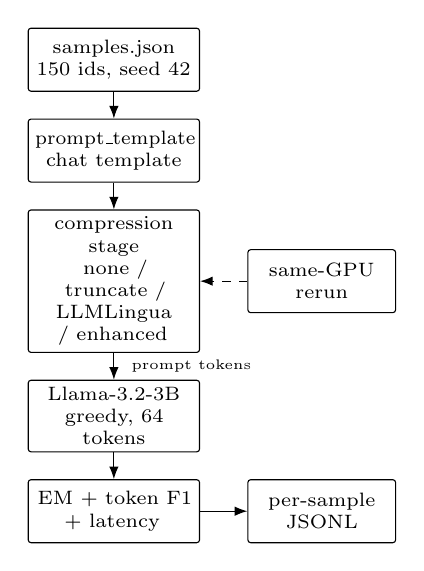
\begin{tikzpicture}[
  font=\scriptsize,
  box/.style={draw, rounded corners=1pt, align=center, inner sep=2.5pt, minimum height=8mm, text width=20mm},
  arr/.style={-{Latex[length=1.6mm]}, line width=0.4pt},
  node distance=3.4mm
]
\node[box] (idx) {samples.json\\150 ids, seed 42};
\node[box, below=of idx] (tmp) {prompt\_template\\chat template};
\node[box, below=of tmp] (comp) {compression stage\\none / truncate /\\LLMLingua / enhanced};
\node[box, below=of comp] (gen) {Llama-3.2-3B\\greedy, 64 tokens};
\node[box, below=of gen] (score) {EM + token F1\\+ latency};
\node[box, right=6mm of score, text width=17mm] (json) {per-sample\\JSONL};
\node[box, right=6mm of comp, text width=17mm] (rerun) {same-GPU\\rerun};
\draw[arr] (idx) -- (tmp);
\draw[arr] (tmp) -- (comp);
\draw[arr] (comp) -- node[right, xshift=1mm, font=\tiny]{prompt tokens} (gen);
\draw[arr] (gen) -- (score);
\draw[arr] (score) -- (json);
\draw[arr, dashed] (rerun) -- (comp);
\end{tikzpicture}
\caption{Data flow shared by all four parts. The frozen contract (sample index,
template, decoding, metric) is drawn on the left; only the compression stage is
replaced between settings. Dashed: the same-GPU rerun replays the five
uncompressed/truncation/LLMLingua stages to make latency comparable.}
\label{fig:system}
\end{figure}

\subsection{Experimental Setup}

Seven result settings are reported, produced by five per-part runs plus one
same-environment rerun (Table~\ref{tab:setup}). Accuracy and token counts come from
the per-part runs, which are the runs each member documented; latency comes from
the rerun, which is the only run in which all five of its settings share one GPU
and one software environment. Part 4 has no rerun counterpart.

\begin{table*}[t]
\centering
\footnotesize
\setlength{\tabcolsep}{6pt}
\begin{tabular}{@{}llll@{}}
\toprule
Setting & Device & Achieved ratio & Result file \\
\midrule
Uncompressed & RTX 3060 & 1.000 & \texttt{part1\_uncompressed/results\_member1.json} \\
Head-tail 2x & Colab T4 & 1.969 & \texttt{part2\_truncation/results\_member2\_2x.json} \\
Head-tail 4x & Colab T4 & 3.820 & \texttt{part2\_truncation/results\_member2\_4x.json} \\
LLMLingua 2x & M5 Pro (MPS) & 2.094 & \texttt{part3\_llmlingua/results\_member3.json} \\
LLMLingua 4x & M5 Pro (MPS) & 3.508 & \texttt{part3\_llmlingua/results\_member3.json} \\
LLMLingua-Enh.\ 2x & Colab CUDA & 2.144$^{\dagger}$ & \texttt{part4\_llmlingua\_enhanced/results\_member4.json} \\
LLMLingua-Enh.\ 4x & Colab CUDA & 4.133$^{\dagger}$ & \texttt{part4\_llmlingua\_enhanced/results\_member4.json} \\
\midrule
Rerun (5 settings) & RTX 3060 & separately measured & \texttt{results\_same\_machine/} \\
\bottomrule
\end{tabular}
\caption{Experimental setup. Ratios are means of per-example achieved whole-prompt ratios.\\
$^{\dagger}$Whole-prompt reduction measured directly: 53.3\% and 76.1\%.}
\label{tab:setup}
\end{table*}

\subsection{Evaluation Protocol}
\label{sec:protocol}

F1 is the primary metric; EM is reported but is too strict to discriminate
between settings on sentence-length gold answers. Because all methods answer the
same items, we do not compare independent means. For each contrast we compute the
per-sample difference $\Delta_i = F1^{\text{after}}_i - F1^{\text{before}}_i$,
average it over the 150 items, and form a 95\% confidence interval as
$\bar{\Delta} \pm 1.96\,\mathrm{SE}(\Delta)$, where $\mathrm{SE}$ is the standard
error of the paired differences. These are approximate, unadjusted exploratory intervals; interval exclusion of zero is reported for this evaluation, without a benchmark-wide inference. Pairing removes the between-question difficulty variance,
which is large here (the per-setting standard deviation of F1 is about 0.29), and
tightens the intervals by factors of approximately 1.37--1.95 relative to an unpaired standard-error calculation for the twelve reported historical contrasts. Latency is compared only within the rerun; per-part latency
values are reported for completeness but never used in a claim, and Part 4's
timings are quoted alone. The largest absolute per-setting F1 difference between the historical and same-environment runs is 0.0076.

% ---------------------------------------------------------------------------
\section{Results and Evaluation}

\subsection{Main Results}

Table~\ref{tab:main} reports the seven settings. Three patterns are visible
immediately. First, F1 decreases monotonically with the compression ratio in all
three compressed families: 0.4296 $\rightarrow$ 0.4065 $\rightarrow$ 0.3620 for
truncation, 0.4296 $\rightarrow$ 0.2626 $\rightarrow$ 0.2207 for LLMLingua, and
0.4296 $\rightarrow$ 0.3070 $\rightarrow$ 0.2794 for the enhanced variant. Second,
the size of that decrease differs enormously between families: at $2\times$
truncation loses 5.4\% of relative F1 while LLMLingua loses 38.9\%. Third, Exact
Match collapses much faster than F1 and is essentially uninformative for the LLMLingua settings (0 to 2 exact matches of 150) and low for truncation (10 to 11 of 150), which is why we treat F1 as the
measurement and EM as a sanity check.

\begin{table*}[t]
\centering
\footnotesize
\setlength{\tabcolsep}{4.2pt}
\resizebox{\textwidth}{!}{%
\begin{tabular}{@{}lrrrrrrrr@{}}
\toprule
Method & $n$ & EM & F1 & F1 sd & Mean prompt tokens & Token reduction & Compress.\ s & Total\ s \\
\midrule
Uncompressed            & 150 & 0.0933 & \textbf{0.4296} & 0.2910 & 6{,}966.8 & ---     & 0.000  & 4.65 \\
Head-tail $2\times$     & 150 & 0.0733 & 0.4065 & 0.2931 & 3{,}523.1 & 49.4\%  & 0.019  & 5.82 \\
Head-tail $4\times$     & 150 & 0.0667 & 0.3620 & 0.2978 & 1{,}801.2 & 74.1\%  & 0.018  & 3.55 \\
LLMLingua $2\times$     & 150 & 0.0067 & 0.2626 & 0.2675 & 3{,}308.1 & 52.5\%  & 10.816 & 13.84 \\
LLMLingua $4\times$     & 150 & 0.0133 & 0.2207 & 0.2396 & 1{,}961.6 & 71.8\%  & 9.846  & 11.98 \\
LLMLingua-Enh.\ $2\times$ & 150 & 0.0000 & 0.3070 & 0.2571 & 3{,}254.1 & 53.3\% & 16.913 & 19.64 \\
LLMLingua-Enh.\ $4\times$ & 150 & 0.0067 & 0.2794 & 0.2559 & 1{,}663.0 & 76.1\% & 14.654 & 16.48 \\
\bottomrule
\end{tabular}%
}
\caption{Main results, all seven settings, per-part runs. Accuracy and token counts
are the numbers used in all claims. The two latency columns come from four
different machines and are shown for completeness only; comparable latencies are
in Table~\ref{tab:rerun}.}
\label{tab:main}
\end{table*}

\begin{figure*}[t]
\centering
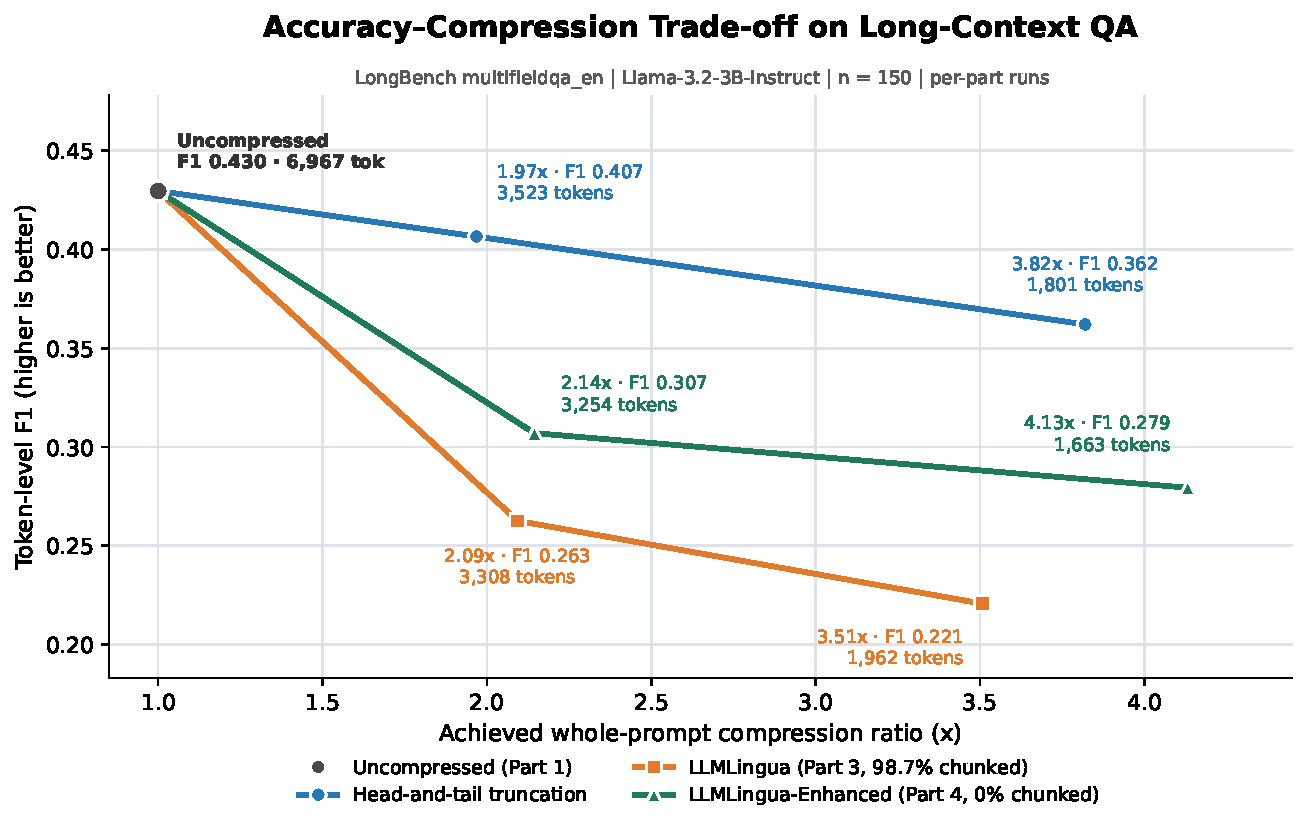
\includegraphics[width=0.66\textwidth]{accuracy_compression_tradeoff.pdf}
\caption{F1 against the mean achieved whole-prompt compression ratio for all seven historical settings.
Truncation stays close to the uncompressed baseline at both ratios; the LLMLingua
family degrades sharply, and the enhanced variant sits between the two but below
truncation at nearby achieved budgets.}
\label{fig:tradeoff}
\end{figure*}

\begin{table}[t]
\centering
\footnotesize
\setlength{\tabcolsep}{3pt}
\begin{tabular}{@{}lrrl@{}}
\toprule
Contrast & $\overline{\Delta F1}$ & 95\% CI & Verdict \\
\midrule
Uncomp.\ $\rightarrow$ HT $2\times$ & $-0.0231$ & $[-0.057,+0.011]$ & n.s. \\
Uncomp.\ $\rightarrow$ HT $4\times$ & $-0.0676$ & $[-0.107,-0.028]$ & sig. \\
Uncomp.\ $\rightarrow$ LL $2\times$ & $-0.1670$ & $[-0.208,-0.127]$ & sig. \\
Uncomp.\ $\rightarrow$ LL $4\times$ & $-0.2090$ & $[-0.250,-0.168]$ & sig. \\
Uncomp.\ $\rightarrow$ Enh.\ $2\times$ & $-0.1226$ & $[-0.162,-0.083]$ & sig. \\
Uncomp.\ $\rightarrow$ Enh.\ $4\times$ & $-0.1503$ & $[-0.192,-0.108]$ & sig. \\
HT $2\times$ $\rightarrow$ LL $2\times$ & $-0.1440$ & $[-0.186,-0.102]$ & sig. \\
HT $4\times$ $\rightarrow$ LL $4\times$ & $-0.1414$ & $[-0.183,-0.100]$ & sig. \\
LL $2\times$ $\rightarrow$ Enh.\ $2\times$ & $+0.0444$ & $[+0.013,+0.076]$ & \textbf{gain} \\
LL $4\times$ $\rightarrow$ Enh.\ $4\times$ & $+0.0587$ & $[+0.025,+0.093]$ & \textbf{gain} \\
HT $2\times$ $\rightarrow$ Enh.\ $2\times$ & $-0.0995$ & $[-0.142,-0.057]$ & sig. \\
HT $4\times$ $\rightarrow$ Enh.\ $4\times$ & $-0.0827$ & $[-0.128,-0.037]$ & sig. \\
\bottomrule
\end{tabular}
\caption{Paired per-sample F1 contrasts on the same 150 items (per-part runs).
HT = head-and-tail truncation, LL = LLMLingua, Enh.\ = LLMLingua-Enhanced,
n.s.\ = interval includes zero.}
\label{tab:paired}
\end{table}

\subsection{RQ1: Accuracy versus Compression Ratio}

Figure~\ref{fig:tradeoff} plots F1 against the mean achieved whole-prompt compression ratio. The
historical mean F1 falls across the two requested settings inside every compressed family. This describes these aggregate means, not per-example monotonicity. The magnitudes, however, are not comparable. Going from no
compression to $4\times$ costs 0.0676 F1 with truncation but 0.2090 with
LLMLingua, a threefold difference at the same nominal budget.

The paired contrasts (Table~\ref{tab:paired}) sharpen this. The truncation loss at
$2\times$ has an approximate paired interval that includes zero
($-0.0231$, $[-0.057,+0.011]$), so no reliable loss is detectable in the per-part runs (the same-machine rerun shows a marginal loss; see Threats to Validity); at $4\times$ the interval excludes zero
($-0.0676$) but is still modest. Both LLMLingua settings lose far more, and the
enhanced variant loses less than LLMLingua while remaining clearly below the
baseline. Notably, the per-sample spread of F1 remains broad across settings (0.24--0.30). Similar standard deviations alone do not identify whether losses are concentrated in a subset of examples.

\subsection{RQ2: LLMLingua versus Truncation at Comparable Token Budgets}
\label{sec:rq2}

In the historical comparisons, both LLMLingua variants have lower mean F1 than head-and-tail truncation at nearby, but unequal, achieved budgets. At $2\times$ the gap is $-0.1440$
$[-0.186,-0.102]$, and at $4\times$ it is $-0.1414$ $[-0.183,-0.100]$; both
approximate paired intervals exclude zero in this evaluation. They do not remove implementation or hardware confounding. The budgets are close but not identical: at $4\times$ LLMLingua keeps 1{,}962 prompt tokens against 1{,}801 for truncation (about 9\% more), so fewer total tokens cannot explain that particular gap; at $2\times$ it keeps 3{,}308 against 3{,}523 (about 6\% fewer); the enhanced variant keeps 3{,}254 and 1{,}663.

Part 4 explores a possible explanation while changing several factors together. Part 3 had to compress 296 of
300 rows in chunks because Phi-2 cannot hold a full LongBench document, which makes
it a different algorithm from the paper's whole-prompt version. Part 4 removes
chunking completely (0 of 300 rows) by using a long-context compressor, and it does
improve: $+0.0444$ $[+0.013,+0.076]$ at $2\times$ and $+0.0587$
$[+0.025,+0.093]$ at $4\times$ over Part 3, both significant. But the improvement
recovers only about 31\% of the $2\times$ gap and 42\% of the $4\times$ gap, and
the enhanced variant remains significantly below truncation
($-0.0995$ and $-0.0827$). These improvements are consistent with several possible mechanisms, including
the absence of independent compression chunks, but they do not test chunking in
isolation. The 31\% and 42\% values are descriptive fractions of the observed F1
gap recovered by the combined Part 4 variant, not causal bounds.

Part 4 did not reach its design goal of overtaking truncation: it stays 0.0995 and 0.0827 F1 below Part 2 and about 0.108 and 0.101 below its own targets. Two caveats belong with this conclusion. Part 4 changes five factors at once
(compressor size, question conditioning, sentence-level filtering, context length,
4-bit weights), so neither the size nor the sign of the isolated chunking effect is identified. And the targets recorded in the project plan (F1 $\approx 0.415$ and $0.380$) were
not met, so it is a negative result for \emph{this} implementation of the paper's
claim, not evidence that LLMLingua cannot work.

\subsection{Additional Released-Recipe and Matched-Budget Evaluation}
\label{sec:matched}

A later full-split experiment used the authors' published LLMLingua inference
recipe with the author-referenced \texttt{vicgalle/alpaca-7b} checkpoint,
\texttt{context\_budget=*2}, \texttt{iterative\_size=100}, original LLMLingua
ranking, and separate instruction, context and question inputs. Both models used
fp16 without quantization. Source-preserving paragraph units of at most 512
compressor tokens adapted the single document to the context-list interface.
The checkpoint revision and model-loading checks were recorded; the trained output
head was restored from its legacy weight key and verified exactly. This transfers
the released inference recipe to LongBench/Llama-3.2 chat evaluation; it does not
recreate the original datasets, target models, alignment training or full protocol.

All 150 ids were included at both requested settings. Verified pilot rows were
reused without changing the recipe. The existing head-tail algorithm was also
evaluated on the same MPS target at each LLMLingua output's actual prompt budget,
selected using token counts only. Of 300 pairs, 288 match exactly and 12 differ
by one token. These results are separate from the historical Phi-2 and Qwen rows.

\begin{table}[t]
\centering\footnotesize
\setlength{\tabcolsep}{3pt}
\begin{tabular}{lrrrr}
\toprule
Requested & LL F1 & HT F1 & LL tokens & Ratio \\
\midrule
$2\times$ & 0.2396 & 0.3875 & 1{,}966.4 & 3.5375 \\
$4\times$ & 0.2174 & 0.3494 & 1{,}113.4 & 5.9006 \\
\bottomrule
\end{tabular}
\caption{Released-recipe Alpaca evaluation, 150 ids per setting. HT is matched
to the actual LL prompt budget; Ratio is the mean per-example whole-prompt ratio.}
\label{tab:matched}
\end{table}

The paired LLMLingua-minus-head-tail F1 differences are $-0.1479$ with approximate
95\% CI $[-0.1912,-0.1046]$ and $-0.1320$ with CI $[-0.1731,-0.0909]$.
These unadjusted exploratory intervals favor truncation in this setting. They
provide a direct budget-controlled comparison that the historical nominal-ratio
tables do not. The paired $4\times$-minus-$2\times$ LLMLingua difference is
$-0.0222$, CI $[-0.0458,+0.0014]$; this mean decline is not clearly separated
from zero by that interval.

Achieved ratios exceed the requested labels. Every context unit survives coarse
filtering at the $2\times$ setting, and output falls below the recorded fine-stage
budget. The precise implementation cause has not been isolated. The 7B
compressor is larger than the 3B target; stage timings with pilot reuse are not a
dedicated speed benchmark. Historical common-environment seconds must not be
assigned to this experiment.

\subsection{RQ3: End-to-End Latency}

Table~\ref{tab:rerun} gives the only latencies we compare, all from one RTX 3060
with one software stack. Truncation reduces total latency by 43.5\% at $2\times$
and 65.7\% at $4\times$, because it removes tokens and adds little overhead: its
compression stage takes 0.02\,s. LLMLingua at $2\times$ is 43.9\% \emph{slower}
than the uncompressed baseline (13.57\,s against 9.43\,s): generation time does fall
from 9.40\,s to 6.03\,s, but compression adds 7.50\,s, more than the saving. At
$4\times$ the picture improves slightly (10.76\,s total) but the setting is still
slower than doing nothing.

\begin{table}[t]
\centering
\footnotesize
\setlength{\tabcolsep}{3.2pt}
\begin{tabular}{@{}lrrrrrr@{}}
\toprule
Method & $n$ & F1 & Prompt & Gen.\ s & Comp.\ s & Total\ s \\
\midrule
Uncompressed        & 150 & 0.4350 & 6{,}966.8 & 9.403 & ---    & 9.43 \\
Head-tail $2\times$ & 150 & 0.3990 & 3{,}523.1 & 5.291 & 0.020  & 5.32 \\
Head-tail $4\times$ & 150 & 0.3633 & 1{,}801.2 & 3.209 & 0.019  & 3.23 \\
LLMLingua $2\times$ & 150 & 0.2569 & 3{,}309.1 & 6.032 & 7.496  & 13.57 \\
LLMLingua $4\times$ & 150 & 0.2221 & 1{,}962.8 & 4.034 & 6.711  & 10.76 \\
\bottomrule
\end{tabular}
\caption{Same-environment rerun on a single RTX 3060 (\texttt{run\_all.py}). All
latency claims in this report come from this table. Part 4 is excluded because its
compressor could not be loaded on this host.}
\label{tab:rerun}
\end{table}

Part 4 has mean compression times of 16.9\,s and 14.7\,s and total times of
19.6\,s and 16.5\,s on its own host. This establishes substantial compression
overhead, but there is no uncompressed run on that host from which to measure
net savings. We therefore draw no cross-method latency conclusion for Part 4.
Within the earlier common-environment experiment, only truncation reduces total
latency. This result applies to the historical Phi-2 implementation, not to every
LLMLingua-family method or hardware configuration.

\subsection{Qualitative Analysis}

Four illustrative paired cases from the committed result files show possible failure modes;
they are regenerated by a script with explicit selection rules, so they are not
cherry-picked by hand.

\emph{Case 1 --- lossless compression of a salient fact.} Asked when \emph{Weep
Not, Child} was first published, the gold answer appears at 0.2\% of the document
and is repeated later. LLMLingua answers correctly at both ratios (F1 1.000), as
does the baseline. Truncation scores 0.800 at $2\times$ because it adds a name, and 1.000 at $4\times$. When the fact is short, salient and redundant, token-level
deletion costs nothing.

\emph{Case 2 --- compression succeeds where position fails.} For a question about
the infall rate and gas density in a magnetised accretion model, the evidence sits
at 65.1\% of the document, outside both kept regions. Truncation at $2\times$ and
$4\times$ collapses to F1 0.182 and answers that ``the text does not provide a
direct comparison''; LLMLingua keeps the numerical relation (F1 0.667 and 0.788).
This illustrates a case where LLMLingua answers better than the positional baseline.

\emph{Case 3 --- a precise detail is deleted.} Asked for a publication date,
truncation answers ``7 March 2023'' correctly at both ratios, LLMLingua at
$2\times$ drops the year (F1 0.923) and at $4\times$ answers that the date is not
mentioned (F1 0.133). The date is near the start of the document, which is consistent with information loss during compression. A controlled token-restoration test would be needed to isolate the cause.

\emph{Case 4 --- a plausible distractor survives.} Asked in which electorate Simon
English was elected, the baseline and truncation answer ``Wallace''; LLMLingua
answers ``Clutha-Southland'' at both ratios. The source contains both names,
with a temporal relation needed to distinguish them. The output error is consistent with weakened relational evidence, but does not by itself prove which deletion caused it.

These illustrative cases show both successes and failures. They motivate hypotheses about missing details and relations, but do not establish their frequency or explain the aggregate gap causally.

\subsection{Answer-Position Analysis of the Truncation Baseline}
\label{sec:position}

Truncation deletes the middle of the document, so its errors should concentrate
where the evidence is. To test this we locate each gold answer in the
\emph{original} document and map it to token offsets with the tokenizer's offset
mapping, then compare the span with the kept head and tail. A sample is
\texttt{kept\_head} or \texttt{kept\_tail} when an occurrence of the answer lies
fully inside the kept region, \texttt{partial} when an occurrence overlaps a
boundary, \texttt{dropped\_middle} when every occurrence falls in the removed
middle, and \texttt{not\_found} when no occurrence can be located (yes/no answers,
inferred answers). Matching is normalised exact matching first; when that fails we
take the best sliding window by content-word overlap (threshold 0.6) and mark the
row \texttt{fuzzy}. This yields 46 exact, 87 fuzzy and 17 unmatched locations,
identical at both ratios because the location does not depend on the ratio. The
fuzzy locations are approximate, so all position results are correlational.

\begin{table}[t]
\centering
\footnotesize
\setlength{\tabcolsep}{3.4pt}
\begin{tabular}{@{}llrrr@{}}
\toprule
Ratio & Zone & $n$ & Mean F1 & Mean EM \\
\midrule
$2\times$ & kept\_head      & 85 & 0.4921 & 0.1176 \\
$2\times$ & kept\_tail      & 16 & 0.3768 & 0.0000 \\
$2\times$ & partial         & 1  & 0.2069 & 0.0000 \\
$2\times$ & dropped\_middle & 31 & 0.2259 & 0.0323 \\
$2\times$ & not\_found      & 17 & 0.3481 & 0.0000 \\
\midrule
$4\times$ & kept\_head      & 63 & 0.5109 & 0.1587 \\
$4\times$ & kept\_tail      & 11 & 0.3762 & 0.0000 \\
$4\times$ & partial         & 3  & 0.3501 & 0.0000 \\
$4\times$ & dropped\_middle & 56 & 0.2006 & 0.0000 \\
$4\times$ & not\_found      & 17 & 0.3351 & 0.0000 \\
\bottomrule
\end{tabular}
\caption{Answer-position analysis of the truncation baseline: mean F1 by zone.
Group sizes are reported with every number because \texttt{partial} and
\texttt{kept\_tail} are small.}
\label{tab:zone}
\end{table}

\begin{table}[t]
\centering
\footnotesize
\setlength{\tabcolsep}{4pt}
\begin{tabular}{@{}llrrr@{}}
\toprule
Ratio & Pooled zone & $n$ & Mean F1 & 95\% CI \\
\midrule
$2\times$ & Kept (head+tail) & 101 & 0.474 & $[0.416, 0.531]$ \\
$2\times$ & Partial          & 1   & 0.207 & --- \\
$2\times$ & Dropped          & 31  & 0.226 & $[0.154, 0.311]$ \\
$4\times$ & Kept (head+tail) & 74  & 0.491 & $[0.419, 0.564]$ \\
$4\times$ & Partial          & 3   & 0.350 & $[0.205, 0.429]$ \\
$4\times$ & Dropped          & 56  & 0.201 & $[0.149, 0.255]$ \\
\bottomrule
\end{tabular}
\caption{Pooled zones with 95\% bootstrap confidence intervals
(\texttt{answer\_position\_stats}). Intervals for Kept and Dropped do not overlap
at either ratio. These intervals are retained from the committed summary; their generating script, seed and replicate count are unavailable for independent reproduction.}
\label{tab:pooled}
\end{table}

\begin{figure}[t]
\centering
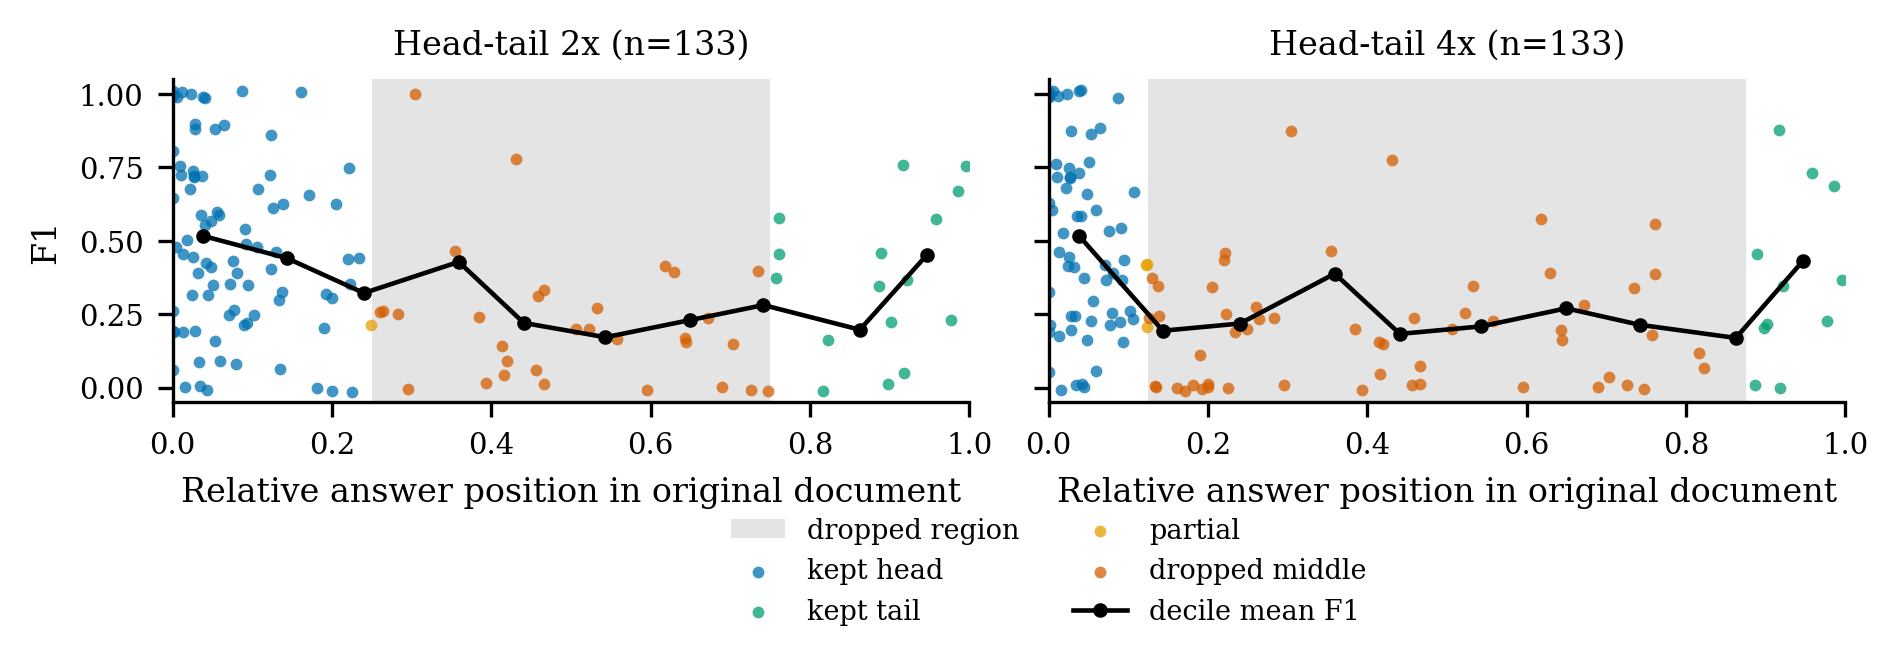
\includegraphics[width=\columnwidth]{fig_answer_position_scatter.png}
\caption{F1 against the relative position of the gold answer in the original
document. The removed middle region is shaded; decile means trace the same pattern
as the zone analysis.}
\label{fig:scatter}
\end{figure}

\begin{figure}[t]
\centering
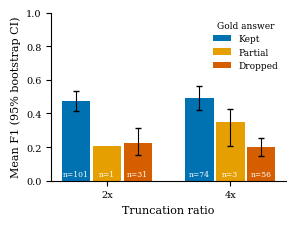
\includegraphics[width=\columnwidth]{fig_f1_by_answer_zone.png}
\caption{Mean F1 by pooled answer zone at $2\times$ and $4\times$. The kept groups have higher mean F1 than the dropped groups. Membership differs across ratios, so the bars do not represent within-example changes.}
\label{fig:zonef1}
\end{figure}

\begin{figure}[t]
\centering
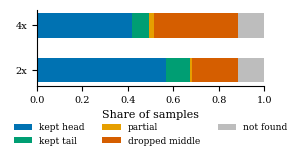
\includegraphics[width=0.86\columnwidth]{fig_zone_share.png}
\caption{Share of samples in each zone. The dropped-middle share rises from 21\%
to 37\% between $2\times$ and $4\times$, which is associated with the lower mean F1 at the $4\times$ setting.}
\label{fig:zoneshare}
\end{figure}

Tables~\ref{tab:zone}--\ref{tab:pooled} and Figures~\ref{fig:scatter}--\ref{fig:zoneshare}
give three findings. First, F1 is clearly lower when the gold answer falls in the
removed middle: 0.226 against 0.474 at $2\times$, and 0.201 against 0.491 at
$4\times$, with non-overlapping intervals in the committed bootstrap summary. Second, the dropped-middle group grows from 31 to 56 of 150 examples
(21\% to 37\%) between settings. Mean F1 is 0.474 and 0.491 in the respective
kept groups and 0.226 and 0.201 in the dropped groups. Group membership changes
with the ratio, so these averages do not measure a within-example treatment effect.
Third, many approximate answer locations are near the start, which is consistent
with a positional heuristic retaining useful evidence in this dataset.

For a fairer reference, uncompressed mean F1 on exactly the same kept ids is
0.4320 at $2\times$ and 0.4477 at $4\times$, compared with truncation's 0.4738
and 0.4909. On the dropped ids it is 0.4838 and 0.4190, compared with 0.2259
and 0.2006. These are descriptive paired-subset means. They do not establish
that retained-answer errors come only from the generator: fuzzy localization can
be wrong and supporting evidence can still be removed.

\subsection{Discussion}

Why does a perplexity-based compressor lose to a baseline that knows nothing about
the question? We offer four hypotheses that are consistent with our data but were not tested directly.

\emph{Fragmentation.} Token-level deletion removes words whose loss is locally
predictable, which is not the same as removing words whose loss is harmless for a
downstream answer. Relations expressed as ``the seat was later renamed
Clutha-Southland'' survive entity deletion as two unrelated entities (Case 4),
while short high-information tokens such as years and numbers disappear (Case 3).
Truncation is coarse but syntactically coherent: what it keeps, it keeps whole.

\emph{Target-model sensitivity.} LLMLingua's published numbers use much larger
target models. A possible explanation is that a 3B model is sensitive to grammatical and referential damage from token deletion. We did not vary target size or measure fluency, so this mechanism remains untested. Our results are
therefore a statement about small open-weight deployments, and they do not refute
the paper's results with its original target models.

\emph{Prompt geometry.} In our setting the question follows the context and is
never compressed, and the context is one long article whose evidence is not uniformly spread. Both favour the positional baseline: evidence tends to appear
early (85 of 150 answers in the head zone), so a degenerate policy keeps the right
region most of the time. In a setting where evidence is uniformly spread, the positional baseline might degrade; whether the gap shrinks requires a separate experiment.

\emph{Cost accounting.} Iterative token scoring requires multiple model
computations. Its overhead exceeded generation savings in the historical
common-environment run. Other target sizes, prompt lengths, implementations or
reuse patterns could change this balance and require separate measurements.

\subsection{Threats to Validity}

\emph{Hardware heterogeneity.} Greedy decoding can vary with the execution environment;
we observed that 12 of 150 uncompressed answers differ word for word between two
GPUs under greedy decoding, with a mean F1 difference of 0.0053. This is one observed rerun difference, not a general noise floor.
All latency claims are restricted to the single-GPU rerun.

\emph{Significance flips.} The uncompressed $\rightarrow$ head-and-tail $2\times$
contrast is insignificant in the per-part runs ($-0.0231$, $[-0.057,+0.011]$) and
barely significant in the rerun ($-0.0360$, $[-0.069,-0.003]$). We report it as a
marginal loss at the edge of significance rather than choosing the friendlier run.

\emph{Stale export.} The committed \texttt{results\_table.md} inside
\texttt{results\_same\_machine} was generated from the per-part result files
rather than from the rerun files stored beside it, so it still shows cross-machine
latencies; the authoritative rerun numbers are the ones in Table~\ref{tab:rerun},
regenerated directly from the rerun JSON files.

\emph{Single dataset, model, and hyper-parameter.} One task, one target model, one
head fraction, two ratios. The ``truncation beats compression'' ranking is
established for \texttt{multifieldqa\_en} with Llama-3.2-3B and should not be
generalised to other benchmarks without replication.

\emph{Part 4 is not a clean ablation.} Its gain combines several changes and does not identify a chunking effect; it also has no common-hardware latency measurement, so no cross-method
latency claim involving Part 4 is made.

\emph{Interface deviation.} The \texttt{docs} field is empty in all five result
files, deviating from the interface declared in the plan. This affects all parts
equally, so comparability is preserved, but these answer files alone cannot reconstruct the exact compressed inputs. Stored answers can still be rescored, and separate compression checkpoints retain inputs for Parts 3 and 4.

\emph{Position analysis.} 87 of 150 answer locations come from fuzzy matching, 17
cannot be located, and the analysis is correlational: questions whose evidence
appears early may also be intrinsically easier. Group sizes for
\texttt{partial} and \texttt{kept\_tail} are too small to support separate claims.

% ---------------------------------------------------------------------------
\section{Conclusion}

\subsection{Summary of Findings}

\textbf{RQ1.} Mean F1 decreases across the two requested compression settings in
the historical truncation, Phi-2 and enhanced-Qwen experiments. This is a pattern
in the evaluated means, not a universal or per-example monotonicity claim.
The later Alpaca experiment also has a lower mean at the stronger setting, but
its paired interval includes zero.

\textbf{RQ2.} Historical LLMLingua variants have lower mean F1 than head-tail
truncation at nearby achieved budgets. The combined Qwen variant recovers
31\% and 42\% of the observed Phi-2 deficit; this does not identify or bound
the contribution of chunking alone. In the later actual-budget-matched Alpaca
experiment, LLMLingua obtains F1 0.2396 and 0.2174, compared with 0.3875 and
0.3494 for truncation, with approximate paired intervals favoring truncation.

\textbf{RQ3.} In the earlier same-environment Parts 1--3 experiment, truncation
reduces total latency by 43.5\% and 65.7\%, whereas the chunked Phi-2 variant
increases it by 43.9\% and 14.1\%. Part 4 has no common-hardware control, and
the later Alpaca run is not a dedicated latency benchmark.

For the tested dataset, target model and implementations, head-tail truncation is
therefore a strong practical baseline. This is not a general ranking of all
LLMLingua-family methods or long-context applications. Position analysis is
consistent with early evidence favoring truncation, but fuzzy localization and
changing group membership prevent a causal explanation of the performance gap.

\subsection{Lessons Learned}

Shared prompts and scoring make results comparable, but nominal compression
labels do not guarantee equal actual budgets. Actual token counts, verified
checkpoint loading and explicit implementation boundaries are essential.
Input-token reduction alone does not establish an end-to-end speedup; compression
and generation must be measured together on common hardware. Finally, a negative
result can guide further tests without assigning causes that the experiment did
not isolate. Sentence-only selection, controlled chunking ablations and other
target sizes remain useful future experiments, not demonstrated improvements.

\subsection{Problems and Difficulties}

\emph{Gated model access.} The canonical Llama-3.2 identifier requires accepting a
licence; we standardised on the ungated mirror. Its model card identifies the intended source model; model-card comparison alone does not establish tensor-level weight identity.

\emph{Windows console encoding.} One baseline run crashed at sample 87 because the
console codec could not encode a character in a generated answer. The fix was to
write records as UTF-8 explicitly and to stop printing predictions to the console;
the crash is a reminder that a long unattended run needs I/O that cannot fail on
data.

\emph{Compressor context limit.} Phi-2 cannot hold a 15k-token document, which
forced 1{,}400-token chunked compression and turned Part 3 into a partially
different algorithm. This limitation became a research question and produced the
Part 4 experiment.

\emph{Out-of-memory on Colab.} The T4 nodes forced chunked prefill, a skip-and-retry path for Part 2, and a resumable design; without the JSONL checkpoints, several runs
would have had to start over.

\emph{Environment conflict for Part 4.} The 4-bit Qwen compressor required a
different software stack that could not be installed on the Windows host that ran
the other parts, so Part 4 ran on Colab. This is the reason it has no
same-hardware latency measurement, and it also caused the Windows
commit-limit failure that blocked running it locally.

\emph{Heterogeneous hardware.} Four machines produced the four parts, which cost us
an extra 30-minute rerun before any latency claim could be made.

\subsection{Limitations}

\begin{itemize}
    \item One dataset (\texttt{multifieldqa\_en}, 150 examples), one target model
    (3B), one head fraction, two ratios: the ranking is not established beyond
    this configuration.
    \item F1 is lexical overlap, not semantic correctness; EM is near zero for
    sentence-length gold answers and is used only as a sanity check.
    \item Generation is capped at 64 tokens, which penalises long gold answers.
    \item Historical Part 3 is a chunked adaptation of LLMLingua, and Part 4 is a
    multi-factor variant; neither is the paper's exact configuration.
    \item Part 4 has no same-hardware latency measurement, and its accuracy gain is
    confounded.
    \item The position analysis relies on fuzzy matching for 87 of 150 answers and
    is correlational.
    \item Greedy decoding is not bit-exact across GPUs, so small differences between runs require cautious interpretation.
\end{itemize}

\subsection{Future Work}

The most direct extension is to repeat the position analysis for the compressed
settings, so that the failure modes of Case 3 and Case 4 can be counted rather
than illustrated: does compression shift errors towards questions whose answer is
a date, a number, or a relation between two entities? Second, the confounding in
Part 4 should be removed by an ablation that changes one factor at a time
(de-chunking only, then question conditioning only) on a fixed compressor size.
Third, the latency result should be completed by running all four parts, including
Part 4, on one GPU with one environment, and by measuring time-to-first-token in
addition to total time. Fourth, the study should be extended to a larger target
model and to benchmarks with uniformly distributed evidence, where the positional
baseline is weakest; if the gap shrinks there, the conclusion of this report is a
statement about small models and early-evidence datasets rather than about
LLMLingua.

% ---------------------------------------------------------------------------
\section{Use of Generative AI}

Generative AI tools were used for literature organisation, for drafting and
editing prose, for LaTeX formatting and figure layout, and for code assistance and
debugging. Answer metrics were recomputed from stored predictions and references; result JSONs are authoritative where summaries disagree. The later Alpaca inputs, predictions, matched-baseline results and verification scripts accompany the report in the repository. Experimental outputs come from model inference, not invented values. The position bootstrap intervals are retained from the group summary and have not been independently regenerated because the generating script is unavailable. Final submission requires group review.

% ---------------------------------------------------------------------------
\begin{thebibliography}{9}

\bibitem[Bai et al.(2024)]{bai-etal-2024-longbench}
Yushi Bai, Xin Lv, Jiajie Zhang, Hongchang Lyu, Jiankai Tang, Zhidian Huang, Zhengxiao Du, Xiao Liu, Aohan Zeng, Lei Hou, Yuxiao Dong, Jie Tang, and Juanzi Li. 2024.
\newblock LongBench: A bilingual, multitask benchmark for long context understanding.
\newblock In \emph{Proceedings of the 62nd Annual Meeting of the Association for Computational Linguistics (Volume 1: Long Papers)}, pages 3119--3137.

\bibitem[Jiang et al.(2023)]{jiang-etal-2023-llmlingua}
Huiqiang Jiang, Qianhui Wu, Chin-Yew Lin, Yuqing Yang, and Lili Qiu. 2023.
\newblock LLMLingua: Compressing prompts for accelerated inference of large language models.
\newblock In \emph{Proceedings of the 2023 Conference on Empirical Methods in Natural Language Processing}, pages 13358--13376.

\bibitem[Jiang et al.(2024)]{jiang-etal-2024-longllmlingua}
Huiqiang Jiang, Qianhui Wu, Xufang Luo, Dongsheng Li, Chin-Yew Lin, Yuqing Yang, and Lili Qiu. 2024.
\newblock LongLLMLingua: Accelerating and enhancing LLMs in long context scenarios via prompt compression.
\newblock In \emph{Proceedings of the 62nd Annual Meeting of the Association for Computational Linguistics (Volume 1: Long Papers)}, pages 1658--1677.

\bibitem[Kwiatkowski et al.(2019)]{kwiatkowski-etal-2019-natural}
Tom Kwiatkowski, Jennimaria Palomaki, Olivia Redfield, Michael Collins, Ankur Parikh, Chris Alberti, Danielle Epstein, Illia Polosukhin, Jacob Devlin, Kenton Lee, Kristina Toutanova, Llion Jones, Matthew Kelcey, Ming-Wei Chang, Andrew M. Dai, Jakob Uszkoreit, Quoc Le, and Slav Petrov. 2019.
\newblock Natural Questions: A benchmark for question answering research.
\newblock \emph{Transactions of the Association for Computational Linguistics}, 7:453--466.

\bibitem[Li et al.(2023)]{li-etal-2023-compressing}
Yucheng Li, Bo Dong, Frank Guerin, and Chenghua Lin. 2023.
\newblock Compressing context to enhance inference efficiency of large language models.
\newblock In \emph{Proceedings of the 2023 Conference on Empirical Methods in Natural Language Processing}, pages 6342--6353.

\bibitem[Li et al.(2025)]{li-etal-2025-prompt-survey}
Zongqian Li, Yinhong Liu, Yixuan Su, and Nigel Collier. 2025.
\newblock Prompt compression for large language models: A survey.
\newblock In \emph{Proceedings of the 2025 Conference of the Nations of the Americas Chapter of the Association for Computational Linguistics: Human Language Technologies (Volume 1: Long Papers)}, pages 5807--5823.

\bibitem[Liu et al.(2024)]{liu-etal-2024-lost}
Nelson F. Liu, Kevin Lin, John Hewitt, Ashwin Paranjape, Michele Bevilacqua, Fabio Petroni, and Percy Liang. 2024.
\newblock Lost in the middle: How language models use long contexts.
\newblock \emph{Transactions of the Association for Computational Linguistics}, 12:157--173.

\end{thebibliography}

\end{document}
